\باب{طاقتی تسلسل سے سادہ تفرقی مساوات کا حل۔اعلٰی تفاعل}
گزشتہ بابوں میں \ترچھا{مستقل عددی سر} والے خطی سادہ تفرقی مساوات کے حل حاصل کیے گئے جو \اصطلاح{بنیادی تفاعل} تھے۔بنیاد تفاعل مثلاً \عددی{\sin 3t}، \عددی{t^6} اور \عددی{e^{2t}} کو آپ \اصطلاح{علم الاحصاء}\فرہنگ{علم الاحصاء}\حاشیہب{calculus}\فرہنگ{calculus} سے جانتے ہیں۔\اصطلاح{متغیر عددی سر} والے سادہ تفرقی مساوات کے حل نسبتاً مشکل سے حاصل ہوتے ہیں اور یہ حل غیر بنیادی تفاعل ہو سکتے ہیں۔ \اصطلاح{لیژانڈر}، \اصطلاح{بیسل} اور \اصطلاح{بیش ہندسی} مساوات اس نوعیت کے سادہ تفرقی مساوات ہیں۔یہ مساوات اور ان کے حل \اصطلاح{لیژانڈر تفاعل}، \اصطلاح{بیسل تفاعل} اور \اصطلاح{بیش ہندسی تفاعل} انجینئری میں نہایت اہم کردار ادا کرتے ہیں لہٰذا ان مساوات کو حل کرنے کے دو مختلف ترکیبوں پر غور کیا جائے گا۔

پہلی ترکیب میں مساوات کا حل \اصطلاح{طاقتی تسلسل}\فرہنگ{تسلسل!طاقتی}\فرہنگ{طاقتی!تسلسل}\حاشیہب{power series}\فرہنگ{series!power}\فرہنگ{power series} \عددی{a_0+a_1x+a_2x^2+a_3x^3+\cdots} کی صورت میں حاصل کیا جاتا ہے لہٰذا اس کو \اصطلاح{ترکیب طاقتی تسلسل}\فرہنگ{ترکیب طاقتی تسلسل}\فرہنگ{طاقتی تسلسل!ترکیب}\حاشیہب{power series method}\فرہنگ{power series method} کہتے ہیں۔

طاقتی تسلسل کو \عددی{\ln x} یا کسری طاقت \عددی{x^r} سے ضرب دیتے ہوئے دوسری ترکیب حاصل ہوتی ہے جو \اصطلاح{ترکیب فروبنیوس}\فرہنگ{ترکیب فروبنیوس}\فرہنگ{فروبنیوس!ترکیب}\حاشیہب{Frobenius method}\فرہنگ{Frobenius method} کہلاتی ہے۔جہاں خالصتاً طاقتی تسلسل کی صورت میں حل لکھنا ممکن نہ ہو وہاں ترکیب فروبنیوس کار آمد ثابت ہوتا ہے لہٰذا یہ ترکیب زیادہ عمومی ہے۔

ایسے تمام اعلٰی حل جنہیں آپ علم الاحصاء سے نہیں جانتے  \اصطلاح{اعلٰی تفاعل}\فرہنگ{اعلٰی تفاعل}\حاشیہب{higher functions or special functions}\فرہنگ{higher functons}\فرہنگ{special functions} کہلاتے ہیں۔
%================

\حصہ{ترکیب طاقتی تسلسل}
\موٹا{متغیر} عددی سر والے خطی سادہ تفرقی مساوات کو عموماً \اصطلاح{ترکیب طاقتی تسلسل} سے حل کرتے ہوئے طاقتی تسلسل کی صورت میں حل حاصل کیا جاتا ہے۔اس طاقتی تسلسل سے حل کی قیمت دریافت کی جا سکتی ہے، حل کا خط کھینچا جا سکتا ہے، کلیات ثابت کیے جا سکتے ہیں اور اسی طرح دیگر معلومات حاصل کی جا سکتی ہے۔اس حصے میں طاقتی تسلسل کے تصور پر غور کیا جائے گا۔

علم الاحصاء سے ہم جانتے ہیں کہ \عددی{x-x_0} کا طاقتی تسلسل درج ذیل ہے
\begin{align}\label{مساوات_بیسل_تسلسل_الف} 
\sum_{m=0}^{\infty} a_m(x-x_0)^m=a_0+a_1(x-x_0)+a_2(x-x_0)^2+a_3(x-x_0)^3+\cdots
\end{align}
جس میں \عددی{x} متغیر ہے جبکہ \عددی{a_0}،\عددی{a_1}،\عددی{a_2}،\نقطے تسلسل کے \اصطلاح{عددی سر}\فرہنگ{عددی سر}\حاشیہب{coefficients}\فرہنگ{coefficients} کہلاتے ہیں اور \عددی{x_0} مستقل مقدار ہے جو تسلسل کا \اصطلاح{وسط}\فرہنگ{وسط}\حاشیہب{center}\فرہنگ{center} کہلاتا ہے۔جیسا مساوات \حوالہ{مساوات_بیسل_تسلسل_الف} میں دکھایا گیا ہے، تسلسل کو عموماً \اصطلاح{علامت مجموعہ}\فرہنگ{علامت مجموعہ}\حاشیہب{summation}\فرہنگ{summation} (\عددی{\sum}) کی مدد سے مختصراً لکھا جاتا ہے جس میں \اصطلاح{اشاریہ}\فرہنگ{اشاریہ}\حاشیہب{index}\فرہنگ{index} مختلف اجزاء کی نشاندہی کرتی ہے۔درج بالا مساوات میں \عددی{m} بطور اشاریہ استعمال کیا گیا ہے۔علامت مجموعہ کے نیچے \عددی{m=0} اور اس کے اوپر \عددی{\infty} مجموعے کی پہلے اور آخری جزو کی نشاندہی کرتے ہیں۔  تسلسل کا وسط صفر \عددی{(x_0=0)} ہونے کی صورت میں \عددی{x} کا طاقتی تسلسل
\begin{align} \label{مساوات_بیسل_تسلسل_ب} 
\sum_{m=0}^{\infty} a_m x^m=a_0+a_1 x+a_2 x^2+a_3 x^3+\cdots
\end{align}
 حاصل ہوتا ہے۔ہم فرض کرتے ہیں کہ تمام متغیرات اور مستقل مقدار \موٹا{حقیقی} ہے۔

طاقتی تسلسل سے مراد مساوات \حوالہ{مساوات_بیسل_تسلسل_الف} یا مساوات \حوالہ{مساوات_بیسل_تسلسل_ب} کی تسلسل ہے جس میں \عددی{x-x_0} (یا \عددی{x}) کا منفی طاقت یا کسری طاقت \موٹا{نہیں} پایا جاتا۔
%=============

\ابتدا{مثال}\quad \اصطلاح{مکلارن} تسلسل درحقیقت میں طاقتی تسلسل ہیں\\
\begin{align*}
\frac{1}{1-x}&=\sum_{m=0}^{\infty}x^m=1+x+x^2+x^3+\cdots\quad \quad (\abs{x}<1,\, \text{\RL{ہندسی تسلسل}})\\
e^x&=\sum_{m=0}^{\infty} \frac{x^m}{m!}=1+x+\frac{x^2}{2!}+\frac{x^3}{3!}+\cdots\\
\sin x&=\sum_{m=0}^{\infty} \frac{(-1)^m x^{2m+1}}{(2m+1)!}=x-\frac{x^3}{3!}+\frac{x^5}{5!}-+\cdots\\
\cos x&=\sum_{m=0}^{\infty}\frac{(-1)^m x^{2m}}{(2m)!}=1-\frac{x^2}{2!}+\frac{x^4}{4!}-+\cdots
\end{align*}
\انتہا{مثال}
%======================

\جزوحصہء{ترکیب طاقتی تسلسل کا تصور}
آپ نے درج بالا مثال میں کئی بنیادی تفاعل کے طاقتی تسلسل دیکھے۔یوں آپ دیکھ سکتے ہیں کہ خطی سادہ تفرقی مساوات کا حل طاقتی تسلسل کی صورت میں لکھا جا سکتا ہے۔ ایک مثال کی مدد سے اس ترکیب کو سمجھتے ہیں۔
%===========

\ابتدا{مثال}\quad طاقتی تسلسل حل \\
تفرقی مساوات \عددی{y'+y=0} کو ترکیب طاقتی تسلسل سے حل کریں۔

حل:پہلی قدم میں حل کو طاقتی تسلسل کی صورت میں لکھ کر
\begin{align}\label{مساوات_بیسل_طاقتی_تسلسل_حل_الف}
y=a_0+a_1x+a_2x^2+a_3x^3+\cdots=\sum_{m=0}^{\infty} a_m x^m
\end{align}
تسلسل کا جزو با جزو تفرق لیتے ہیں۔
\begin{align}\label{مساوات_بیسل_طاقتی_تسلسل_حل_ب}
y'=a_1+2a_2x+3a_3x^2+\cdots=\sum_{m=1}^{\infty} ma_mx^{m-1}
\end{align}
انہیں دیے گئے تفرقی مساوات میں پر کرتے ہوئے
\begin{align*}
(a_0+a_1x+a_2x^2+a_3x^3+\cdots)+(a_1+2a_2x+3a_3x^2+\cdots)=0
\end{align*}
\عددی{x} کی طاقت کے لحاظ سے ترتیب دیتے ہیں۔
\begin{align*}
(a_0+a_1)+(a_1+2a_2)x+(a_2+3a_3)x^2+\cdots=0
\end{align*}
اس مساوات کا دایاں ہاتھ صفر کے برابر ہے لہٰذا بائیں ہاتھ تمام اجزاء بھی صفر کے برابر ہوں گے۔
\begin{align*}
a_0+a_1=0,\quad a_1+2a_2=0, \quad a_2+3a_3=0
\end{align*}
ان سے درج ذیل لکھا جا سکتا ہے۔
\begin{align*}
a_1=-a_0,\quad a_2=-\frac{a_1}{2}=\frac{a_0}{2},\quad a_3=-\frac{a_2}{3}=-\frac{a_0}{3!}
\end{align*}
ان عددی سر کو استعمال کرتے ہوئے  حل \حوالہ{مساوات_بیسل_طاقتی_تسلسل_حل_الف} لکھتے ہیں جو قوت نمائی تفاعل \عددی{e^{-x}} کی مکلارن تسلسل ہے۔
\begin{align*}
y=a_0(1-x+\frac{x^2}{2!}-\frac{x^3}{3!}+-\cdots)=a_0 e^{-x}
\end{align*}
یہاں آپ  \عددی{y''+y=0} کو ترکیب طاقتی تسلسل سے حل کرتے ہوئے حل \عددی{y=a_0\cos x+a_1\sin x} حاصل کریں۔
\انتہا{مثال}
%=================

اب اس ترکیب کی عمومی استعمال پر غور کرتے ہیں جبکہ اگلے مثال کے بعد اس کا جواز پیش کرتے ہیں۔پہلی قدم میں ہم خطی سادہ تفرقی مساوات
\begin{align}\label{مساوات_بیسل_طاقتی_عمومی_مساوات_الف}
y''+p(x)y'+q(x)y=0
\end{align}
میں \عددی{p(x)} اور \عددی{q(x)} کو \عددی{x} کے تسلسل کی صورت  (اور اگر حل \عددی{x-x_0} کی تسلسل کی صورت میں درکار ہو تب انہیں \عددی{x-x_0} کی تسلسل کی صورت) میں لکھتے ہیں۔ اگر \عددی{p(x)} اور \عددی{q(x)} اذ خود  \ترچھا{کثیر رکنی}  ہوں تب پہلی قدم میں کچھ کرنے کی ضرورت نہیں ہے۔ دوسری قدم میں حل کو مساوات \حوالہ{مساوات_بیسل_طاقتی_تسلسل_حل_الف} کی طرح تصور کرتے ہوئے  مساوات \حوالہ{مساوات_بیسل_طاقتی_تسلسل_حل_ب} کی طرح \عددی{y'} اور درج ذیل \عددی{y''} لکھتے ہوئے
\begin{align}\label{مساوات_بیسل_طاقتی_تسلسل_حل_پ}
y''=2a_2+3\cdot 2 a_3x+4\cdot 3 a_4x^2+5\cdot 4 a_5 x^3+\cdots=\sum_{m=2}^{\infty} m(m-1)a_mx^{m-2}
\end{align}
مساوات \حوالہ{مساوات_بیسل_طاقتی_عمومی_مساوات_الف} میں پر کریں۔تیسری قدم میں \عددی{x} کی طاقت کے لحاظ سے ترتیب دیتے ہوئے، مستقل مقدار سے شروع کرتے ہوئے، باری باری \عددی{x^1}، \عددی{x^2}، \نقطے کے عددی سر کو صفر کے برابر پر کریں۔یوں تمام عددی سر کو \عددی{a_0} اور \عددی{a_1} کی صورت میں حاصل کرتے ہوئے اصل حل لکھیں۔
%===============

\ابتدا{مثال}\شناخت{مثال_بیسل_کلیہ_توالی_الف} \quad ایک مخصوص \اصطلاح{لیژانڈر مساوات}\\
درج ذیل مساوات کروی تشاکل خاصیت رکھتی ہے۔اس کو حل کریں۔
\begin{align*}
(1-x^2)y''-2xy'+2y=0
\end{align*} 
حل:مساوات \حوالہ{مساوات_بیسل_طاقتی_تسلسل_حل_الف}، مساوات \حوالہ{مساوات_بیسل_طاقتی_تسلسل_حل_ب} اور مساوات \حوالہ{مساوات_بیسل_طاقتی_تسلسل_حل_پ} کو درج بالا میں پر کرتے ہوئے
\begin{multline*}
(1-x^2)(2a_2+3\cdot 2 a_3x+4\cdot 3 a_4x^2+5\cdot 4 a_5x^3+6\cdot 5 a_6x^4\cdots)\\
-2x(a_1+2a_2x+3a_3x^2+4a_4x^3+\cdots)\\
+2(a_0+a_1x+a_2x^2+a_3x^3+a_4x^4+\cdots)=0
\end{multline*}
یعنی
\begin{multline*}
(2a_2+3\cdot 2 a_3x+4\cdot 3 a_4x^2+5\cdot 4a_5 x^3+6\cdot 5 a_6x^4\cdots)\\
+(-2a_2 x^2-3\cdot 2 a_3x^3-4\cdot 3a_4 x^4-5\cdot 4a_5x^5-\cdots)\\
+(-2a_1x-2\cdot 2a_2x^2-3\cdot 2a_3x^3-4\cdot 2 a_4x^4-\cdots)\\
+(2a_0+2a_1x+2a_2x^2+2a_3x^3+2a_4x^4+\cdots)=0
\end{multline*}
ملتا ہے جس کو \عددی{x} کی طاقت کے لحاظ سے ترتیب دیتے ہیں۔
\begin{multline*}
(2a_2+2a_0)+(3\cdot 2 a_3-2a_1+2a_1)x\\
+(4\cdot 3 a_4-2a_2-2\cdot 2a_2+2a_2)x^2\\
+(5\cdot 4a_5-3\cdot 2 a_3-3\cdot 2a_3+2a_3)x^3\\
+(6\cdot 5a_6-4\cdot 3a_4-4\cdot 2a_4+2a_4)x^4+\cdots=0
\end{multline*}
مستقل مقدار سے شروع کرتے ہوئے باری باری \عددی{x}، \عددی{x^2}، \عددی{x^3}، \نقطے کے عددی سر کو صفر کے برابر پر کرتے ہوئے بالترتیب \عددی{a_2}،\عددی{a_3}،\عددی{a_4}، \نقطے کو \عددی{a_0} اور \عددی{a_1} کی صورت میں حاصل کرتے ہیں۔
\begin{align*}
a_2&=-a_0\\
a_3&=0\\
a_4&=\frac{a_2}{3}=-\frac{a_0}{3}\\
a_5&=\frac{a_3}{2}=0\quad \text{\RL{(چونکہ \عددی{a_3=0} ہے)}}\\
a_6&=\frac{3}{5}a_4=-\frac{a_0}{5}
\end{align*}
ان عددی سروں کو مساوات \حوالہ{مساوات_بیسل_طاقتی_تسلسل_حل_الف} میں پر کرتے ہوئے حل لکھتے ہیں
\begin{align*}
y=a_1x+a_0(1-x^2-\frac{1}{3}x^4-\frac{1}{5}x^6-\cdots)
\end{align*}
جس میں \عددی{a_0} اور \عددی{a_1} اختیاری مستقل ہیں۔یوں درج بالا عمومی حل دو عدد حل \عددی{x} اور \عددی{1-x^2-\tfrac{1}{3}x^4-\cdots} پر مشتمل ہے جو  \اصطلاح{لیژانڈر کثیر رکنی}\فرہنگ{لیژانڈر!کثیر رکنی تفاعل}\حاشیہب{Legendre polynomials}\فرہنگ{Legendre!polynomial} \عددی{P_n(x)} اور \اصطلاح{لیژانڈر تفاعل}\فرہنگ{لیژانڈر!تفاعل}\حاشیہب{Legendre function}\فرہنگ{Legendre!function} \عددی{Q_n(x)} کے رکن  ہیں۔یہاں \عددی{x=P_1(x)} اور 
\عددی{1-x^2-\frac{1}{3}x^4-\frac{1}{5}x^6-\cdots=-Q_1(x)} ہیں جہاں منفی علامت روایتی ہے۔\عددی{n} لیژانڈر کثیر رکنی اور لیژانڈر تفاعل کا \اصطلاح{درجہ}\فرہنگ{درجہ!لیژانڈر}\حاشیہب{order}\فرہنگ{order!Legendre} کہلاتا ہے۔یہاں \عددی{n=1} ہے لہٰذا لیژانڈر کثیر رکنی اور لیژانڈر تفاعل کا درجہ \عددی{1} ہے۔
\انتہا{مثال}
%===================

\جزوحصہء{نظریہ طاقتی تسلسل}
مساوات \حوالہ{مساوات_بیسل_تسلسل_الف} کے چند ارکان کا جزوی مجموعہ \عددی{s_n(x)} لکھتے ہیں جس کو \عددی{n} \اصطلاح{جزوی مجموعہ}\فرہنگ{جزوی مجموعہ}\حاشیہب{nth partial sum}\فرہنگ{partial sum} کہتے ہیں۔ 
\begin{align}
s_n(x)=a_0+a_1(x-x_0)+a_2(x-x_0)^2+\cdots +a_n (x-x_0)^n
\end{align}
یہاں \عددی{n=0,1,2,\cdots} ممکن ہے۔مساوات \حوالہ{مساوات_بیسل_تسلسل_الف} سے \عددی{s_n(x)} منفی کرنے سے بقایا \عددی{R_n(x)} حاصل ہوتا ہے جس کو \عددی{a_n(x-x_0)^n} کے بعد  مساوات \حوالہ{مساوات_بیسل_تسلسل_الف} کا \اصطلاح{بقایا}\فرہنگ{بقایا}\حاشیہب{remainder}\فرہنگ{remainder} کہتے ہیں۔
\begin{align}
R_n(x)=a_{n+1}(x-x_0)^{n+1}+a_{n+2}(x-x_0)^{n+2}+\cdots
\end{align}
یوں ہندسی تسلسل 
\begin{align*}
1+x+x^2+x^3+x^4+\cdots
\end{align*}
کے \اصطلاح{جزوی مجموعے} اور نظیری \اصطلاح{بقایا} درج ذیل ہوں گے۔
\begin{align*}
s_0&=1, &R_0=x+x^2+x^3+\cdots\\
s_1&=1+x,&R_1=x^2+x^3+x^4+\cdots\\
s_2&=1+x+x^2, &R_2=x^3+x^4+x^5+\cdots
\end{align*}
اس طرح مساوات \حوالہ{مساوات_بیسل_تسلسل_الف} کے ساتھ ہم جزوی مجموعوں \عددی{s_0(x)}، \عددی{s_1(x)}،\عددی{s_2(x)} \نقطے کی ترتیب وابستہ کرتے ہیں۔اگر کسی \عددی{x=x_1} کے لئے جزوی مجموعوں کی ترتیب  مرتکز ہو مثلاً 
\begin{align*}
\lim_{n \to \infty} s_n(x_1)=s(x_1)
\end{align*}
تب  ہم کہتے ہیں کہ نقطہ \عددی{x=x_1} پر تسلسل \حوالہ{مساوات_بیسل_تسلسل_الف} \اصطلاح{مرکوز}\فرہنگ{مرتکز}\حاشیہب{converge}\فرہنگ{converge} ہے جبکہ \عددی{s(x_1)} کو تسلسل \حوالہ{مساوات_بیسل_تسلسل_الف} کی \اصطلاح{قیمت}\فرہنگ{طاقتی تسلسل!قیمت}\حاشیہب{value or sum}\فرہنگ{power series!value or sum} یا \اصطلاح{مجموعہ}\فرہنگ{طاقتی تسلسل!مجموعہ} کہتے ہیں جس کو درج ذیل لکھا جاتا ہے۔
\begin{align*}
s(x_1)=\sum_{m=0}^{\infty} a_m(x_1-x_0)^m
\end{align*}
اس طرح کسی بھی \عددی{n} کے لئے ہم درج ذیل لکھ سکتے  ہیں۔
\begin{align}\label{مساوات_بیسل_تسلسل_مجموعہ_الف}
s(x_1)=s_n(x_1)+R_n(x_1)
\end{align}
اس کے برعکس اگر \عددی{s_0(x)}، \عددی{s_1(x)}، \عددی{s_2(x)}، \نقطے کی ترتیب غیر مرکوز ہو تب ہم کہتے ہیں کہ نقطہ \عددی{x=x_1} پر مساوات \حوالہ{مساوات_بیسل_تسلسل_الف} \اصطلاح{منفرج}\فرہنگ{منفرج}\حاشیہب{divergent}\فرہنگ{divergent} ہے۔

مرکوز تسلسل کی صورت میں، کسی بھی مثبت \عددی{\epsilon} کے لئے  ایسا \عددی{N} (جس کی قیمت \عددی{\epsilon} پر منحصر ہے) پایا جاتا ہے کہ ہم تمام \عددی{n>N} کے لئے   مساوات \حوالہ{مساوات_بیسل_تسلسل_مجموعہ_الف} سے درج ذیل لکھ سکتے ہیں۔ 
\begin{align}\label{مساوات_بیسل_مرتکز_حدود}
\abs{R_n(x_1)}=\abs{s(x_1)-s_n(x_1)} < \epsilon \quad \quad \text{\RL{تمام \عددی{n>N}}}
\end{align}
جیومیٹریائی طور (شکل \حوالہ{شکل_مساوات_بیسل_مرتکز_حدود} دیکھیں) پر اس کا مطلب ہے کہ \عددی{s_n(x_1)} جہاں \عددی{n>N} ہے \عددی{s(x_1)-\epsilon} اور \عددی{s(x_1)+\epsilon} کے درمیان پایا جاتا ہے۔عملاً اس کا مطلب ہے کہ مرکوز تسلسل کی صورت  میں \عددی{x_1} پر  مساوات \حوالہ{مساوات_بیسل_تسلسل_الف} کا مجموعہ \عددی{s(x_1)} تقریباً \عددی{s_n(x_1)} کے برابر ہو گا۔مزید یہ کہ \عددی{s(x_1)} اور \عددی{s_n(x_1)} میں فرق کو ہم \عددی{n} بڑھا کر جتنا کم بنانا چاہیں بنا سکتے ہیں۔
\begin{figure}
\centering
\begin{tikzpicture}
\draw(-\x-\x/2,0)--(\x+\x/2,0);
\draw(-\x,-\y/16)node[below]{$s(x_1)-\epsilon$}--++(0,\y/8)coordinate (kL);
\draw(0,-\y/16)node[below]{$s(x_1)$}--++(0,\y/8)coordinate(kM);
\draw(\x,-\y/16)node[below]{$s(x_1)+\epsilon$}--++(0,\y/8)coordinate (kR);
\draw[gray] (kL)++(0,\y/16)--++(0,\y/8)coordinate[pos=0.5](kLA);
\draw[gray] (kM)++(0,\y/16)--++(0,\y/8)coordinate[pos=0.5](kMA);
\draw[gray] (kR)++(0,\y/16)--++(0,\y/8);
\draw[stealth-stealth] (kLA)--++(\x,0)node[pos=0.5,fill=white]{$\epsilon$};
\draw[stealth-stealth] (kMA)--++(\x,0)node[pos=0.5,fill=white]{$\epsilon$};
\end{tikzpicture}
\caption{غیر مساوات \حوالہ{مساوات_بیسل_مرتکز_حدود} کی شکل۔}
\label{شکل_مساوات_بیسل_مرتکز_حدود}
\end{figure}

طاقتی تسلسل کہاں مرکوز ہوتی ہے؟ تسلسل \حوالہ{مساوات_بیسل_تسلسل_الف} میں \عددی{x=x_0} پر  \عددی{a_0} کے علاوہ تمام اجزاء صفر ہو جاتے ہیں لہٰذا تسلسل کی قیمت \عددی{a_0} ہو گی۔یوں \عددی{x=x_0} پر تسلسل \عددی{a_0} پر مرکوز ہوتی ہے۔ کبھی کبھار \عددی{x} کی واحد اسی قیمت پر تسلسل مرتکز ہو گا۔ اگر \عددی{x} کے دیگر قیمتوں کے لئے بھی تسلسل مرتکز ہو تب \عددی{x} کی یہ قیمتیں \اصطلاح{ارتکازی وقفہ}\فرہنگ{ارتکازی وقفہ}\فرہنگ{وقفہ!ارتکازی}\حاشیہب{convergence interval}\فرہنگ{interval!convergence} کہلاتا ہے۔ یہ وقفہ محدود ہو سکتا ہے۔محدود وقفہ جس کا وسط \عددی{x_0} ہے کو شکل \حوالہ{شکل_مساوات_بیسل_مرتکز_محدود_وقفہ} میں دکھایا گیا ہے۔یوں طاقتی تسلسل \حوالہ{مساوات_بیسل_تسلسل_الف} ارتکازی وقفے کے اندر تمام \عددی{x} پر مرکوز ہو گا یعنی درج ذیل مساوات پر پورا اترنے والے \عددی{x} پر تسلسل مرکوز ہو گا
\begin{align}\label{مساوات_بیسل_ارتکازی_وقفہ}
\abs{x-x_0}<R
\end{align}
جبکہ \عددی{\abs{x-x_0}>R} پر تسلسل منفرج ہو گا۔ارتکازی وقفہ لامتناہی بھی ہو سکتا ہے اور ایسی صورت میں طاقتی تسلسل \عددی{x} کی تمام قیمتوں پر مرکوز ہو گا۔
\begin{figure}
\centering
\begin{tikzpicture}
\draw(-\x-\x/2,0)--(\x+\x/2,0);
\draw(-\x,-\y/16)node[below]{$x_0-R$}--++(0,\y/8)coordinate (kL);
\draw(0,-\y/16)node[below]{$x_0$}--++(0,\y/8)coordinate(kM);
\draw(\x,-\y/16)node[below]{$x_0+R$}--++(0,\y/8)coordinate (kR);
\draw[gray] (kL)++(0,\y/16)--++(0,\y/2)coordinate[pos=0.9](kL);
\draw[gray] (kM)++(0,\y/16)--++(0,\y/8)coordinate[pos=0.5](kMA);
\draw[gray] (kR)++(0,\y/16)--++(0,\y/2);
\draw[stealth-stealth] (kMA)--++(-\x,0)node[pos=0.5,fill=white]{$R$};
\draw[stealth-stealth] (kMA)--++(\x,0)node[pos=0.5,fill=white]{$R$};
\draw[stealth-stealth] (kL)node[left]{منفرج}--++(2*\x,0)node[pos=0.5,fill=white]{مرکوزیت}node[right]{منفرج};
\end{tikzpicture}
\caption{ارتکازی وقفہ \حوالہ{مساوات_بیسل_ارتکازی_وقفہ} جس کا وسط \عددی{x_0} ہے۔}
\label{شکل_مساوات_بیسل_مرتکز_محدود_وقفہ}
\end{figure}

شکل \حوالہ{شکل_مساوات_بیسل_مرتکز_محدود_وقفہ} میں \عددی{R} \اصطلاح{رداس ارتکاز}\فرہنگ{رداس!ارتکاز}\فرہنگ{ارتکاز!رداس}\حاشیہب{convergence radius}\فرہنگ{convergence!radius}\فرہنگ{radius!convergence} کہلاتا ہے۔(مخلوط طاقتی تسلسل کی صورت میں ارتکازی وقفہ گول ٹکیا ہوتا ہے جس کا رداس \عددی{R} ہو گا)۔ اگر تسلسل تمام \عددی{x} پر مرکوز ہو تب ہم \عددی{R = \infty} یعنی \عددی{\tfrac{1}{R}=0} لکھتے ہیں۔

رداس ارتکاز کی قیمت کو تسلسل کے عددی سر استعمال کرتے ہوئے  درج ذیل کلیات سے حاصل کیا جا سکتا ہے، پس شرط یہ ہے کہ ان کلیات میں حد (\عددی{\lim}) موجود اور غیر صفر ہو۔اگر یہ حد لامتناہی ہو تب تسلسل \حوالہ{مساوات_بیسل_تسلسل_الف} صرف وسط \عددی{x_0} پر مرکوز ہو گا۔
\begin{align}
R&=\frac{1}{\lim\limits_{m \to \infty} \sqrt[m]{\abs{a_m}}}\\
R&=\frac{1}{\lim\limits_{m \to \infty} \abs{\frac{a_{m+1}}{a_m}}}
\end{align}
%=====================
\ابتدا{مثال}\شناخت{مثال_بیسل_رداس_ارتکاز_الف}\quad رداس ارتکاز \عددی{\infty}، \عددی{1} اور \عددی{0}\\
تینوں تسلسل میں \عددی{m \to \infty} لیتے ہوئے رداس  ارتکاز  \عددی{R} دریافت کرتے ہیں۔
\begin{align*}
e^x=\sum_{m=0}^{\infty} \frac{x^m}{m!}=1+x+\frac{x^2}{2!}+\cdots,\quad \abs{\frac{a_{m+1}}{a_m}}=\frac{\frac{1}{(m+1)!}}{\frac{1}{m!}}=\frac{1}{m+1} \to 0, \quad R \to \infty\\
\frac{1}{1-x}=\sum_{m=0}^{\infty}x^m=1+x+x^2+\cdots,\quad \abs{\frac{a_{m+1}}{a_m}}=\abs{\frac{1}{1}}=1, \quad R=1\\
\sum_{m=0}^{\infty} m!x^m=1+x+2x^2+\cdots,\quad \abs{\frac{a_{m+1}}{a_m}}=\abs{\frac{(m+1)!}{m!}}=m+1 \to \infty,\quad R \to 0
\end{align*} 
لامتناہی رداس ارتکاس \عددی{R \to \infty} سب سے بہتر اور کارآمد صورت ہے جبکہ \عددی{R=0} بے کار صورت ہے۔عموماً تسلسل کا رداس ارتکاز محدود ہوتا ہے۔
\انتہا{مثال}
%======================

درج بالا مثال میں \عددی{\tfrac{1}{1-x}} کے طاقتی تسلسل کا رداس ارتکاز \عددی{R=1} حاصل ہوا جہاں تسلسل کا وسط \عددی{x_0=0} ہے۔مساوات \حوالہ{مساوات_بیسل_ارتکازی_وقفہ} کے تحت \عددی{\abs{x} <1} کے لئے طاقتی تسلسل تفاعل \عددی{\tfrac{1}{1-x}} کو ظاہر کرتی ہے۔آئیں اس حقیقت کو تفصیل سے دیکھیں۔نقطہ \عددی{x=0.2} پر تفاعل کی قیمت \عددی{\tfrac{1}{1-0.2}=1.25} ہے جبکہ اس کے تسلسل میں \عددی{x=0.2} پر کرتے ہوئے بتدریج ارکان کی تعداد بڑھاتے ہوئے مجموعہ حاصل کرتے ہیں۔
\begin{align*}
1&=1\quad \quad \text{\RL{ایک رکن}}\\
1+0.2&=1.2\\
1+0.2+0.2^2&=1.24\\
1+0.2+0.2^2+0.2^3&=1.248\\
1+0.2+0.2^2+0.2^3+0.2^4&=1.2496\quad \quad \text{\RL{پانچ ارکان}}
\end{align*}
طاقتی تسلسل کے پانچ ارکان کا مجموعہ تفاعل کے اصل قیمت کے \عددی{\tfrac{1.2496}{1.25}\times 100=99.968} فی صد ہے۔آپ دیکھ سکتے ہیں کہ، مجموعہ لیتے ہوئے  ارکان کی تعداد بڑھانے سے تسلسل کی قیمت اصل قیمت پر \اصطلاح{مرکوز} ہوتی ہے۔بالکل اسی طرح رداس ارتکاز کے اندر کسی بھی \عددی{x} پر تسلسل سے تفاعل کی قیمت، اصل قیمت کے قریب سے قریب تر، حاصل کی جا سکتی ہے۔

رداس ارتکاز کے باہر تسلسل منفرج ہے۔آئیں رداس ارتکاز کے باہر \عددی{x=1.2} پر تفاعل اور تسلسل کی قیمت حاصل کریں۔تفاعل کی قیمت \عددی{\tfrac{1}{1-1.2}=-5} حاصل ہوتی ہے جبکہ مجموعہ لیتے ہوئے ارکان کی تعداد بڑھا کر دیکھتے ہیں۔ 
\begin{align*}
1&=1 \\
1+1.2&=2.2\\
1+1.2+1.2^2&=3.64\\
1+1.2+1.2^2+1.2^3&=5.368
\end{align*}
آپ دیکھ سکتے ہیں کہ مجموعے میں ارکان کی تعداد بڑھانے سے تسلسل کا مجموعہ اصل قیمت پر مرکوز ہونے کی بجائے اصل قیمت سے \اصطلاح{منتشر} ہوتا نظر آتا ہے۔یوں رداس ارتکاز کے باہر نقطہ \عددی{x} پر یہ تسلسل اصل تفاعل کو ظاہر نہیں کرتا۔ہم کہتے ہیں کہ رداس ارتکاز کے باہر یہ تسلسل \اصطلاح{منفرج} ہے۔

ہم نے رداس ارتکاز کی اہمیت کو تفاعل \عددی{\tfrac{1}{1-x}} کی مدد سے سمجھا جس کی قیمت ہم تفاعل سے ہی حاصل کر سکتے تھے۔طاقتی تسلسل کی اہمیت اس موقع پر ہو گی جب تفاعل کو کسی بھی بنیادی تفاعل کی صورت میں لکھنا ممکن نہ ہو۔


%=============================
اگر سادہ تفرقی مساوات
\begin{align}\label{مساوات_بیسل_معیاری_تفرقی_مساوات_الف}
y''+p(x)y'+q(x)y=r(x)
\end{align}
میں \عددی{p(x)}، \عددی{q(x)} اور \عددی{r(x)} کے طاقتی تسلسل (ٹیلر تسلسل) پائے جاتے ہوں تب اس مساوات کا طاقتی تسلسل حل پایا جاتا ہے۔ایسا تفاعل \عددی{f(x)} جس کو \عددی{x-x_0} کی ایسی طاقتی تسلسل کی صورت میں لکھنا ممکن ہو جس کا مثبت رداس ارتکاز پایا جاتا ہو، \عددی{x_0} پر \اصطلاح{تحلیلی}\فرہنگ{تحلیلی}\حاشیہب{analytic}\فرہنگ{analytic} کہلاتا ہے۔اس تصور کو استعمال کرتے ہوئے درج ذیل مسئلہ بیان کرتے ہیں جس میں مساوات \حوالہ{مساوات_بیسل_معیاری_تفرقی_مساوات_الف} \موٹا{معیاری صورت} میں ہے یعنی یہ \عددی{y''} سے شروع ہوتا ہے۔اگر دو درجی تفرقی مساوات غیر معیاری صورت میں پایا جاتا ہو، یعنی اس میں \عددی{h(x)y''} پایا جاتا ہو تب مساوات کو \عددی{h(x)} سے تقسیم کرتے ہوئے اس کی معیاری صورت حاصل کریں اور درج ذیل مسئلے میں اس معیاری صورت میں لکھی تفرقی مساوات کو استعمال کریں۔
%=================

\ابتدا{مسئلہ}\شناخت{مسئلہ_بیسل_وجودیت_طاقتی_تسلسل_حل}\quad طاقتی تسلسل حل کی وجودیت\\
اگر مساوات \حوالہ{مساوات_بیسل_معیاری_تفرقی_مساوات_الف} میں \عددی{p}، \عددی{q} اور \عددی{r} نقطہ \عددی{x=x_0} پر تحلیلی ہوں، تب مساوات \حوالہ{مساوات_بیسل_معیاری_تفرقی_مساوات_الف} کا ہر حل \عددی{x=x_0} پر تحلیلی ہو گا اور اس کو \عددی{x-x_0} کی ایسی طاقتی تسلسل کی صورت میں لکھنا ممکن ہو گا جس کا رداس ارتکاز \عددی{R>0} ہو۔
\انتہا{مسئلہ}
%==========================

اس مسئلے کا ثبوت آپ کتاب کے آخر میں صفحہ \حوالہصفحہ{حوالہ_بیرونی_مواد} پر حوالہ \cite{حوالہ_کریزگ_الف_گیارہ} سے پڑھ سکتے ہیں۔(دھیان رہے کہ ہو سکتا ہے کہ ایسا نقطہ \عددی{x} محور پر نہ پایا جاتا ہو بلکہ مخلوط سطح پر پایا جاتا ہو۔)

مسئلہ \حوالہ{مسئلہ_بیسل_وجودیت_طاقتی_تسلسل_حل} میں  رداس ارتکاز  کی لمبائی \عددی{x_0} سے کم از کم اس قریب ترین نقطے (یا نقطوں) تک ہو گی جہاں  \عددی{p}، \عددی{q} اور \عددی{r}  میں سے کوئی ایک مخلوط سطح پر غیر تحلیلی ہو۔

%==============================
\جزوحصہء{طاقتی تسلسل پر مختلف عمل}
طاقتی تسلسل کی ترکیب میں ہم طاقتی تسلسلوں کا تفرق، مجموعہ اور  حاصل ضرب لیتے ہوئے، (مثال \حوالہ{مثال_بیسل_کلیہ_توالی_الف} کی طرح) \عددی{x} کی ہر ایک طاقت کے عددی سر کو صفر کے برابر پر کرتے ہوئے تسلسل  کے عددی سر معلوم کرتے ہیں۔یہ چار اعمال درج ذیل وجوہات کی بنا ممکن ہیں۔ ان اعمال کا ثبوت طاقتی تسلسل کے باب میں دیا جائے گا۔

\موٹا{(الف) تسلسل کے ارکان کا تفرق۔}\quad طاقتی تسلسل کے ہر رکن کا انفرادی تفرق لیا جا سکتا ہے۔اگر طاقتی تسلسل
\begin{align*}
y(x)=\sum_{m=0}^{\infty}a_m(x-x_0)^m
\end{align*}
 \عددی{\abs{x-x_0}<R} پر مرکوز ہو، جہاں \عددی{R<0} ہے، تب ہر رکن کا انفرادی تفرق لے کر حاصل تسلسل بھی انہیں \عددی{x} پر مرکوز ہو گا اور یہ تسلسل ان \عددی{x} پر  تفرق  \عددی{y'} کو ظاہر کرے گا۔ 
 \begin{align*}
y'(x)=\sum_{m=1}^{\infty} ma_m(x-x_0)^{m-1}\quad \quad \quad (\abs{x-x_0}<R)
\end{align*}
 اسی طرح دو درجی، تین درجی اور بلند درجی تفرقات بھی حاصل کیے جا سکتے ہیں۔

\موٹا{(ب) تسلسل کے ارکان کا مجموعہ۔}\quad دو عدد طاقتی تسلسل کے ارکان کو جمع کرتے ہوئے ان کا مجموعہ حاصل کیا جا سکتا ہے۔اگر طاقتی تسلسل
\begin{align}\label{مساوات_بیسل_دو_عدد_تسلسل_الف}
\sum_{m=0}^{\infty} a_m(x-x_0)^m\quad \text{اور} \quad \sum_{m=0}^{\infty} b_m(x-x_0)^m
\end{align}
کے رداس ارتکاز مثبت ہوں اور تسلسل کے انفرادی مجموعے \عددی{f(x)} اور \عددی{g(x)} ہوں تب تسلسل
\begin{align*}
\sum_{m=0}^{\infty} (a_m+b_m)(x-x_0)^m
\end{align*}
بھی مرکوز ہو گا اور یہ \عددی{f(x)+g(x)} کو  دونوں تسلسل کے مشترک ارتکازی وقفے کے اندر ہر \عددی{x} پر ظاہر کرے گا۔

\موٹا{(پ) تسلسل کے ارکان کا حاصل ضرب۔}\quad دو عدد طاقتی تسلسل کو رکن با رکن ضرب دیا جا سکتا ہے۔فرض کریں کہ مساوات \حوالہ{مساوات_بیسل_دو_عدد_تسلسل_الف} میں دیے گئے تسلسل کے رداس ارتکاز مثبت ہیں اور ان کے انفرادی مجموعے \عددی{f(x)} اور \عددی{g(x)} ہیں۔اب پہلی تسلسل کے ہر رکن کو دوسری تسلسل کے ہر رکن کے ساتھ ضرب دیتے ہوئے \عددی{x-x_0} کے یکساں طاقت کو اکٹھے کرتے ہوئے حاصل تسلسل
\begin{multline*}
a_0b_0+(a_0b_1+a_1b_0)(x-x_0)+(a_0b_2+a_1b_1+a_2b_0)(x-x_0)^2+\cdots\\
=\sum_{m=0}^{\infty} (a_0b_m+a_1b_{m-1}+\cdots+a_mb_0)(x-x_0)^m
\end{multline*}
مرکوز ہو گا اور \عددی{f(x)g(x)} کو دونوں تسلسل کے مشترک ارتکازی وقفے کے اندر ہر \عددی{x} پر ظاہر کرے گا۔

\موٹا{(ت) تمام عددی سروں کا صفر کے برابر ہونا۔} (طاقتی تسلسل کا مسئلہ  مماثل۔)\quad اگر طاقتی تسلسل کا رداس ارتکاز مثبت اور وقفہ ارتکاز پر تسلسل کا مجموعہ مکمل صفر ہو تب اس تسلسل کا ہر عددی سر صفر کے برابر ہو گا۔
%=================

\حصہء{سوالات}
سوال \حوالہ{سوال_بیسل_رداس_ارتکاز_الف} تا سوال \حوالہ{سوال_بیسل_رداس_ارتکاز_ب} میں رداس ارتکاز دریافت کریں۔

%==========
\ابتدا{سوال}\شناخت{سوال_بیسل_رداس_ارتکاز_الف}\quad
$\sum\limits_{\infty}^{m=0} (m+1)mx^m$\\
جواب:\عددی{R=1}
\انتہا{سوال}
%===========
\ابتدا{سوال}\quad
$\sum\limits_{m=0}^{\infty} \frac{(-1)^mx^m}{k^m}$\\
جواب:\عددی{R=k}
\انتہا{سوال}
%=====================
\ابتدا{سوال}\quad
$\sum\limits_{m=0}^{\infty} \frac{x^{2m+1}}{(2m+1)!}$\\
جواب:\عددی{R = \infty}
\انتہا{سوال}
%=========================
\ابتدا{سوال}\شناخت{سوال_بیسل_رداس_ارتکاز_ب}\quad
$\sum\limits_{m=0}^{\infty}\left(\frac{3}{4}\right)^m x^m$\\
جواب:\عددی{R=\tfrac{4}{3}}
\انتہا{سوال}
%=====================
سوال \حوالہ{سوال_بیسل_قلم_و_کاغذ_الف} تا سوال \حوالہ{سوال_بیسل_قلم_و_کاغذ_ب} کو قلم و کاغذ استعمال کرتے ہوئے ترکیب طاقتی تسلسل حل کریں۔

%===========
\ابتدا{سوال}\شناخت{سوال_بیسل_قلم_و_کاغذ_الف}\quad 
$y'=-2xy$\\
جواب:\عددی{y=a_0(1-x^2+\tfrac{x^4}{2!}-\tfrac{x^6}{3!}+-\cdots)=a_0e^{-x^2}}
\انتہا{سوال}
%====================
\ابتدا{سوال}\quad
$y''+y=0$\\
جواب:\عددی{y=a_0+a_1x-\tfrac{a_0}{2}x^2-\tfrac{a_1}{6}x^3+-\cdots=a_0\cos x+a_1\sin x}
\انتہا{سوال}
%=====================
\ابتدا{سوال}\quad
$(1-x)y'=y$\\
جواب:\عددی{y=a_0(1+x+x^2+x^3+\cdots)=-\tfrac{a_0}{1-x}}
\انتہا{سوال}
%=======================
\ابتدا{سوال}\شناخت{سوال_بیسل_قلم_و_کاغذ_ب}\quad
$xy'-3y=k \quad \text{\RL{جہاں \عددی{k} مستقل مقدار ہے}}$\\
جواب:\عددی{y=cx^3-\tfrac{k}{3}}
\انتہا{سوال}
%========================
سوال \حوالہ{سوال_بیسل_طاقتی_تسلسل_حل_الف} تا سوال \حوالہ{سوال_بیسل_طاقتی_تسلسل_حل_ب} کو ترکیب طاقتی تسلسل سے قلم و کاغذ کی مدد سے حل کریں۔تفرقی مساوات کے بعض اوقات جوابات میں اجزاء کی تعداد لامحدود ہوتی ہے، بعض اوقات جواب میں \عددی{x} کے صرف طاق یا صرف جفت طاقت پائیں جاتے ہیں اور بعض اوقات جواب کی ایک قوسین میں اجزاء کی تعداد محدود ہوتی ہے۔

%============
\ابتدا{سوال}\شناخت{سوال_بیسل_طاقتی_تسلسل_حل_الف}\quad
$y''-y'+xy=0$\\
جواب:\عددی{y=a_0(1-\tfrac{x^3}{6}-\tfrac{x^4}{24}-\tfrac{x^5}{120}+\tfrac{x^6}{240}+\cdots)+a_1(x+\tfrac{x^2}{2}+\tfrac{x^3}{3}-\tfrac{x^4}{24}-\cdots)}
\انتہا{سوال}
%==========================
\ابتدا{سوال}\quad
$y''-y'-xy=0$\\
جواب:\عددی{y=a_0(1+\tfrac{x^3}{6}+\tfrac{x^4}{24}+\tfrac{x^5}{120}+\tfrac{x^6}{144}+\cdots)+a_1(x+\tfrac{x^2}{2}+\tfrac{x^3}{6}+\tfrac{x^4}{8}+\tfrac{x^5}{20}+\cdots)}
\انتہا{سوال}
%==========================
\ابتدا{سوال}\quad
$y''-y'-x^2y=0$\\
جواب:\عددی{y=a_0(1+\tfrac{x^4}{12}+\tfrac{x^5}{60}+\cdots)+a_1(x+\tfrac{x^2}{2}+\tfrac{x^3}{6}+\cdots)}
\انتہا{سوال}
%==========================
\ابتدا{سوال}\quad
$y''-xy'-x^2y=0$\\
جواب:\عددی{y=a_0(1+\tfrac{x^4}{12}+\tfrac{x^6}{90}+\cdots)+a_1(x+\tfrac{x^3}{6}+\tfrac{3x^5}{40}+\cdots)}
\انتہا{سوال}
%==========================
\ابتدا{سوال}\شناخت{سوال_بیسل_طاقتی_تسلسل_حل_ب}\quad
$(1-x^2)y''-2xy'+6y=0$\\
جواب:\عددی{y=a_0(1-3x^2)+a_1(x-\tfrac{2x^3}{3}-\tfrac{x^5}{5}-\cdots)}؛ جواب کی پہلی قوسین لامحدود اجزاء پر مشتمل نہیں ہے۔ 
\انتہا{سوال}
%==========================
\ابتدا{سوال}\quad علامت مجموعہ کی اشاریہ کی منتقلی\\
\عددی{\sum\limits_{s=0}^{\infty}\tfrac{s}{s+1}x^{s+1}} کے پہلے جزو کی نشاندہی \عددی{s=0} کرتا ہے۔اس مجموعے  میں \عددی{k=s+1} پر کرتے ہوئے نیا مجموعہ حاصل کریں جس میں علامت مجموعہ کے اندر \عددی{x^m} پایا جاتا ہو۔اس عمل کو \اصطلاح{منتقلی اشاریہ}\فرہنگ{منتقلی!اشاریہ}\فرہنگ{اشاریہ!منتقلی}\حاشیہب{shifting index}\فرہنگ{index!shifting} کہتے ہیں۔حاصل مجموعے کے پہلے رکن کی نشاندہی کیا کرتی ہے؟

جواب:\عددی{\sum\limits_{k=1}^{\infty}\tfrac{k-1}{k}x^k}؛ پہلا رکن کی نشاندہی \عددی{k=1} کرتا ہے۔
\انتہا{سوال}
%==========================
\ابتدا{سوال}\quad علامت مجموعہ کی اشاریہ کی منتقلی\\
مجموعہ \عددی{\sum\limits_{p=2}^{\infty}\tfrac{p+2}{(p+1)!}x^{p+3}} میں اشاریہ کو یوں منتقل کریں کہ علامت مجموعہ کے اندر \عددی{x^m} ہو۔

جواب:\عددی{\sum\limits_{m=5}^{\infty}\tfrac{m-1}{(m-2)!}x^m}
\انتہا{سوال}
%===========================
سوال \حوالہ{سوال_بیسل_ابتدائی_قیمت_الف} تا سوال \حوالہ{سوال_بیسل_ابتدائی_قیمت_ب} کو ترکیب طاقتی تسلسل کی مدد سے حل کریں۔ابتدائی معلوم کو استعمال کرتے ہوئے، حاصل حل میں \عددی{x^3} تک کے (اور اس رکن کو شامل کرتے ہوئے) اجزاء لیتے ہوئے  مستقل \عددی{a_0} (اور \عددی{a_1}) دریافت کریں۔دیے گئے نقطہ \عددی{x_1} پر مجموعے کی قیمت دریافت کریں۔جوابات میں نقطہ اعشاریہ کے بعد تین ہندسوں تک جواب لکھیں۔

%=================
\ابتدا{سوال}\شناخت{سوال_بیسل_ابتدائی_قیمت_الف}
\begin{align*}
y'+9y=2,\quad y(0)=6,\quad x_1=1
\end{align*}
جوابات:\عددی{y=a_0+(2-9a_0)x+\tfrac{81a_0-18}{2}x^2-\tfrac{243a_0-54}{2}x^3+\cdots}، \\
\عددی{a_0=6}، \عددی{y(1)=-514}
\انتہا{سوال}
%==================
\ابتدا{سوال}
\begin{align*}
y''+4xy'+y=0, \quad y(0)=1,\quad y'(0)=1, \quad x_1=0.1
\end{align*}
جوابات:\عددی{y=a_0(1-\tfrac{x^2}{2}+\tfrac{3x^4}{8}-\cdots)+a_1(x-\tfrac{5x^3}{6}+\cdots)}،\\
 \عددی{a_0=1}، \عددی{a_1=1}، \عددی{y(0.1)=1.094}
\انتہا{سوال}
%==================
\ابتدا{سوال}
\begin{align*}
(1-x^2)y''-2xy'+12y=0, \quad y(0)=0,\quad y'(0)=-\frac{3}{2}, \quad x_1=0.5
\end{align*}
جوابات:\عددی{y=a_0(1-6x^2+3x^4+\cdots)+a_1(x-\tfrac{5x^3}{3})}،\\
 \عددی{a_0=0}، \عددی{a_1=-\tfrac{3}{2}}، \عددی{y(0.5)=-0.437}
\انتہا{سوال}
%==================
\ابتدا{سوال}\شناخت{سوال_بیسل_ابتدائی_قیمت_ب}
\begin{align*}
(x-4)y'=xy,\quad y(1)=5,\quad x_1=2
\end{align*}
جوابات:\عددی{y=a_0(1-\tfrac{x^2}{8}-\tfrac{x^3}{48}+\tfrac{x^4}{256}+\cdots)}، \عددی{a_0=5.827}، \عددی{y(2)=2.307}
\انتہا{سوال}
%===================
\ابتدا{سوال}\شناخت{سوال_بیسل_جزوی_تسلسل}\quad کمپیوٹر کا استعمال\\
طاقتی تسلسل سے تفاعل کی قیمت جزوی تسلسل سے حاصل کی جاتی ہے۔تفاعل \عددی{\sin x} کی تسلسل سے بذریعہ کمپیوٹر،  تسلسل میں اجزاء کی تعداد مختلف لیتے ہوئے سائن کا خط کھینچیں۔آپ دیکھیں گے کے کم  اجزاء لینے سے اصل تفاعل (یعنی \عددی{\sin x}) اور تسلسل میں فرق بہت جلد واضح ہوتا ہے جبکہ زیادہ تعداد میں اجزاء لینے سے یہ فرق دیر بعد نمودار ہوتا ہے۔

جوابات:شکل \حوالہ{شکل_سوال_بیسل_جزوی_تسلسل} میں \عددی{\sin x} کا جزوی مجموعہ \عددی{s_5} اور \عددی{s_7} کے ساتھ موازنہ کیا گیا ہے۔
\begin{figure}
\centering
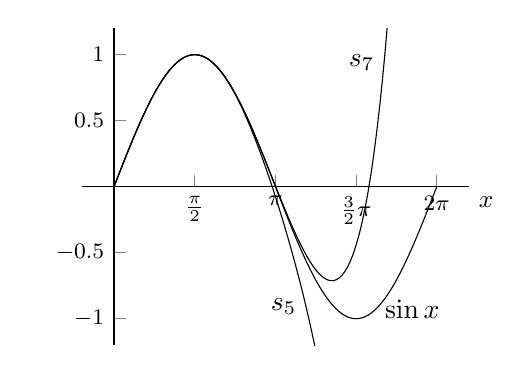
\begin{tikzpicture}
\begin{axis}[small,ymin=-1.2,ymax=1.2,axis lines*=middle,xlabel={$x$},ylabel=\empty,x label style={at={(current axis.right of origin)},anchor=north west},xtick={1.57,3.142,4.71,6.283},xticklabels={$\frac{\pi}{2}$,$\pi$,$\frac{3}{2}\pi$,$2\pi$}]
\addplot[domain=0:2*pi,samples=100]{sin(180/pi*x)}node[pos=0.8,right]{$\sin x$};
\addplot[domain=0:4,samples=100]{x-x^3/6+x^5/120-x^7/5040}node[pos=0.9,left]{$s_5$};
\addplot[domain=0:5.5,samples=100]{x-x^3/6+x^5/120-x^7/5040+x^9/362880}node[pos=0.85,left]{$s_7$};
\end{axis}
\end{tikzpicture}
\caption{سوال \حوالہ{سوال_بیسل_جزوی_تسلسل} کا خط۔\عددی{\sin x} کے علاوہ جزوی مجموعہ \عددی{s_5} اور \عددی{s_7} دکھائے گئے ہیں۔}
\label{شکل_سوال_بیسل_جزوی_تسلسل}
\end{figure}  

\انتہا{سوال}
%======================

\حصہ{لیژانڈر مساوات۔ لیژانڈر کثیر رکنی}
لیژانڈر تفرقی مساوات\فرہنگ{لیژانڈر!تفرقی مساوات}\حاشیہد{فرانسیسی ریاضی دان اڈریان مری لیژانڈر [1752-1833] نے اعلٰی تفاعل، بیضوی تکمل اور اعدادی نظریہ پر کام کیا۔}\حاشیہب{Legendre's equation}\فرہنگ{Legendre!equation}
\begin{align}\label{مساوات_بیسل_لیژانڈر_الف}
(1-x^2)y''-2xy'+n(n+1)y=0\quad \quad (\text{\RL{\عددی{n} مستقل ہے}})
\end{align} 
طبیعیات کے اہم ترین سادہ تفرقی مساوات میں سے ایک ہے جو متعدد مسائل، بالخصوص کرہ کے سرحدی قیمت مسئلوں، میں سامنے آتی ہے۔ 

مساوات میں \اصطلاح{مقدار معلوم}\فرہنگ{مقدار معلوم} \عددی{n} کی قیمت اصل مسئلے کی نوعیت پر منحصر ہوتی ہے لہٰذا مساوات \حوالہ{مساوات_بیسل_لیژانڈر_الف} درحقیقت سادہ تفرقی مساوات کی \اصطلاح{نسل}\فرہنگ{نسل} کو ظاہر کرتی ہے۔ ہم نے لیژانڈر مساوات، جس میں \عددی{n=1} تھا، کو مثال \حوالہ{مثال_بیسل_کلیہ_توالی_الف} میں حل کیا (جس کو ایک مرتبہ دوبارہ دیکھیں)۔ مساوات \حوالہ{مساوات_بیسل_لیژانڈر_الف} کے کسی بھی حل کو \اصطلاح{لیژانڈر تفاعل}\فرہنگ{لیژانڈر!تفاعل}\حاشیہب{Legendre function}\فرہنگ{Legendre!function} کہتے ہیں۔لیژانڈر تفاعل اور ایسے دیگر اعلٰی تفاعل، جو علم الاحصاء میں نہیں پائے جاتے، کے مطالعہ کو \اصطلاح{نظریہ اعلٰی تفاعل}\فرہنگ{نظریہ!اعلٰی تفاعل}\حاشیہب{special functions theory}\فرہنگ{theory!special functions} کہتے ہیں۔دیگر اعلٰی تفاعل اگلے حصوں میں سامنے آئیں گے۔

مساوات \حوالہ{مساوات_بیسل_لیژانڈر_الف} کو \عددی{1-x^2} سے تقسیم کرتے ہوئے تفرقی مساوات کی معیاری صورت حاصل ہوتی ہے جس کے عددی
 سر \عددی{\tfrac{-2x}{1-x^2}} اور \عددی{\tfrac{n(n+1)}{1-x^2}} نقطہ \عددی{x=0} پر \اصطلاح{تحلیلی} تفاعل ہیں لہٰذا لیژانڈر مساوات پر مسئلہ \حوالہ{مسئلہ_بیسل_وجودیت_طاقتی_تسلسل_حل} کا اطلاق ہوتا ہے اور اس کا حل طاقتی تسلسل سے ظاہر کیا جا سکتا ہے۔طاقتی تسلسل
\begin{align}\label{مساوات_بیسل_لیژانڈر_حل_الف}
y=\sum_{m=0}^{\infty}a_mx^m
\end{align}
اور اس کے تفرقات کو مساوات \حوالہ{مساوات_بیسل_لیژانڈر_الف} میں پر کرتے  ہوئے مستقل \عددی{n(n+1)} کو \عددی{k} لکھتے ہوئے
\begin{align*}
(1-x^2)\sum_{m=2}^{\infty}m(m-1)a_mx^{m-2}-2x\sum_{m=1}^{\infty}ma_mx^{m-1}+k\sum_{m=0}^{\infty}a_mx^m=0
\end{align*}
یعنی
\begin{align*}
\sum_{m=2}^{\infty}m(m-1)a_mx^{m-2}-\sum_{m=2}^{\infty}m(m-1)a_mx^m-\sum_{m=1}^{\infty}2ma_mx^{m}+\sum_{m=0}^{\infty}ka_mx^m=0
\end{align*}
حاصل ہوتا ہے۔یہاں آپ مثال \حوالہ{مثال_بیسل_کلیہ_توالی_الف} کی طرح مجموعوں کے چند ابتدائی ارکان لکھ کر آگے بڑھ سکتے ہیں یا پھر درج ذیل طریقہ اختیار کر سکتے ہیں۔ تمام مجموعوں کو  \عددی{x} کی یکساں طاقت کی صورت (\عددی{x^s}) میں لکھنے کی خاطر پہلے مجموعے میں \عددی{s=m-2} یعنی \عددی{m=s+2} پر کرتے ہیں جبکہ بقایا تین مجموعوں میں \عددی{m} کی جگہ \عددی{s} پر کرتے ہیں۔یوں پہلے مجموعے کا پہلا رکن \عددی{m=2} اب \عددی{s=0} ہو گا اور \عددی{a_m} کی جگہ \عددی{a_{s+2}} لکھا جائے گا۔
\begin{align}\label{مساوات_بیسل_لیژانڈر_ب}
\sum_{s=0}^{\infty}(s+2)(s+1)a_{s+2}x^{s}-\sum_{s=2}^{\infty}s(s-1)a_sx^s-\sum_{s=1}^{\infty}2s a_sx^s+\sum_{s=0}^{\infty}ka_s x^s=0
\end{align}
درج بالا مساوات کا دایاں ہاتھ صفر کے برابر ہے لہٰذا مساوات کا بایاں ہاتھ بھی صفر کے برابر ہو گا اور یوں \عددی{x} کے ہر طاقت کے عددی سروں کا مجموعہ صفر کے برابر ہو گا۔یوں \عددی{x^0} کے عددی سر سے شروع کرتے ہوئے باری باری \عددی{x^1}، \عددی{x^2}، \نقطے کے عددی سر صفر کے برابر لکھتے ہیں۔مساوات \حوالہ{مساوات_بیسل_لیژانڈر_ب} کا دوسرا مجموعہ \عددی{x^2} اور تیسرا مجموعہ \عددی{x^1} سے شروع ہوتا ہے لہٰذا ان میں \عددی{x^0} نہیں پایا جاتا ہے۔یوں پہلے اور چوتھے مجموعوں سے \عددی{x^0} کے عددی سر جمع کرتے ہوئے صفر کے برابر پر کرتے ہیں
\begin{align}\label{مساوات_بیسل_لیژانڈر_پ}
2 \cdot 1 a_2+n(n+1)a_0=0
\end{align}
جہاں \عددی{k} کی جگہ واپس \عددی{n(n+1)} لکھا گیا ہے۔ اسی طرح \عددی{x^1} پہلے، تیسرے اور چوتھے مجموعوں میں پایا جاتا ہے جن سے درج ذیل لکھتے ہیں۔
\begin{align}\label{مساوات_بیسل_لیژانڈر_ت}
3\cdot 2 a_3+[-2+n(n+1)]a_1=0
\end{align}
بلند طاقتی اجزاء \عددی{x^2}، \عددی{x^3}، \نقطے تمام مجموعوں میں پائے جاتے ہیں لہٰذا ان کے لئے \عددی{x^s} کے عددی سروں کا مجموعہ لکھتے ہیں۔
\begin{align}\label{مساوات_بیسل_لیژانڈر_ٹ}
(s+2)(s+1)a_{s+2}+[-s(s-1)-2s+n(n+1)]a_s=0
\end{align} 
چکور قوسین \عددی{[\cdots]} کے اندر قوسین کو کھول کر ترتیب دیتے ہوئے درج ذیل لکھا جا سکتا ہے
\begin{align*}
-s(s-1)-2s+n(n+1)&=-s^2+s-2s+n^2+n=n^2-s^2+n-s\\
&=(n-s)(n+s)+n-s\\
&=(n-s)(n+s+1)
\end{align*}
لہٰذا مساوات \حوالہ{مساوات_بیسل_لیژانڈر_ٹ} سے 
\begin{align}\label{مساوات_بیسل_کلیہ_توالی_الف}
a_{s+2}=-\frac{(n-s)(n+s+1)}{(s+2)(s+1)}a_s \quad \quad (s=0,1,\cdots)
\end{align}
حاصل ہوتا ہے جو \اصطلاح{کلیہ توالی}\فرہنگ{کلیہ!توالی}\فرہنگ{توالی کلیہ}\حاشیہب{recurrence relation, recursion formula}\فرہنگ{recursion formula} کہلاتا ہے۔کلیہ توالی کی مدد سے، \عددی{a_0} اور \عددی{a_1} کے علاوہ،  بقایا تمام عددی سر، دو قدم پچھلی عددی سر استعمال کرتے ہوئے دریافت کیے جاتے ہیں۔ یوں \عددی{a_0} اور \عددی{a_1}  اختیاری مستقل ہیں۔ کلیہ توالی کو بار بار استعمال کرتے ہوئے
\begin{gather*}
\begin{aligned}
a_2&=-\frac{n(n+1)}{2!}a_0\\
a_4&=-\frac{(n-2)(n+3)}{4\cdot 3}a_2\\
&=\frac{(n-2)n(n+1)(n+3)}{4!}a_0\\
&\quad\vdots
\end{aligned}\quad\quad
\begin{aligned}
a_3&=-\frac{(n-1)(n+2)}{3!}a_1\\
a_5&=-\frac{(n-3)(n+4)}{5\cdot 4}a_3\\
&=\frac{(n-3)(n-1)(n+2)(n+4)}{5!}a_1\\
&\quad \vdots
\end{aligned}
\end{gather*}
لکھے جا سکتے ہیں جنہیں مساوات \حوالہ{مساوات_بیسل_لیژانڈر_حل_الف} میں پر کرتے ہوئے حل لکھتے ہیں
\begin{align}\label{مساوات_بیسل_حل_لیژانڈر}
y(x)=a_0y_1(x)+a_1y_2(x)
\end{align}
جہاں
\begin{align}\label{مساوات_بیسل_حل_لیژانڈر_الف}
y_1(x)&=1-\frac{n(n+1)}{2!}x^2+\frac{(n-2)n(n+1)(n+3)}{4!}x^4-+\cdots
\end{align}
اور
\begin{align}\label{مساوات_بیسل_حل_لیژانڈر_ب}
y_2(x)&=x-\frac{(n-1)(n+2)}{3!}x^3+\frac{(n-3)(n-1)(n+2)(n+4)}{5!}x^5-+\cdots
\end{align}
ہیں۔یہ تسلسل \عددی{\abs{x}<1} کے لئے مرکوز ہیں۔بعض اوقات تسلسل کا کوئی عددی سر صفر کے برابر حاصل ہوتا ہے اور یوں کلیہ توالی کے تحت اگلے تمام عددی سر بھی صفر ہوں گے اور یوں تسلسل محدود ارکان پر مشتمل ہوتا ہے۔چونکہ مساوات \حوالہ{مساوات_بیسل_حل_لیژانڈر_الف} میں \عددی{x} کے جفت طاقت پائے جاتے ہیں جبکہ مساوات \حوالہ{مساوات_بیسل_حل_لیژانڈر_ب} میں \عددی{x} کے طاق طاقت پائے جاتے ہیں لہٰذا \عددی{\tfrac{y_1}{y_2}} مستقل مقدار نہیں ہو سکتا ہے اور یوں \عددی{y_1} اور \عددی{y_2} آپس میں خطی تعلق نہیں رکھتے لہٰذا یہ خطی طور غیر تابع حل ہیں۔یوں مساوات \حوالہ{مساوات_بیسل_حل_لیژانڈر} کھلے وقفہ \عددی{-1<x<1} پر عمومی حل ہے۔

دھیان رہے کہ \عددی{x=\mp 1} پر \عددی{1-x^2=0} ہو گا لہٰذا سادہ تفرقی مساوات کی معیاری صورت میں عددی سر غیر تحلیلی ہوں گے۔یوں حیرانی کی بات نہیں ہے کہ تسلسل \حوالہ{مساوات_بیسل_حل_لیژانڈر_الف} اور تسلسل \حوالہ{مساوات_بیسل_حل_لیژانڈر_الف} کا ارتکازی وقفہ وسیع نہیں ہے ماسوائے اس صورت میں جب  اجزاء کی تعداد محدود ہونے کی بنا  تسلسل کثیر رکنی کی صورت اختیار کرے۔
%=====================

\جزوحصہء{کثیر رکنی حل۔ لیژانڈر کثیر رکنی \عددی{P_n(x)}}
طاقتی تسلسل کے تخفیف سے کثیر رکنی حاصل ہوتی ہے جس کا حل، ارتکازی شرط کے قید سے آزاد،  تمام \عددی{x} کے لئے پایا جاتا ہے۔ایسے اعلٰی تفاعل جو سادہ تفرقی مساوات کے حل ہوتے ہیں میں یہ صورت عموماً پائی جاتی ہے جن سے مختلف نسل کے اہم کثیر رکنی حاصل ہوتے ہیں۔لیژانڈر مساوات میں \عددی{n} کی قیمت غیر منفی عدد صحیح ہونے کی صورت میں \عددی{s=n} پر مساوات \حوالہ{مساوات_بیسل_کلیہ_توالی_الف} صفر کے برابر ہوتا ہے لہٰذا \عددی{a_{n+2}=0} ہو گا اور یوں \عددی{a_{n+4}=0}، \عددی{a_{n+6}=0}، \نقطے ہوں گے۔جفت \عددی{n} کی صورت میں \عددی{y_1} کثیر رکنی ہو گا جبکہ طاق \عددی{n} کی صورت میں \عددی{y_2} کثیر رکنی ہو گا۔ان کثیر رکنی کو مستقل مقدار سے ضرب دیتے ہوئے \اصطلاح{لیژانڈر کثیر رکنی}\فرہنگ{لیژانڈر!کثیر رکنی}\حاشیہب{Legendre polynomial}\فرہنگ{Legendre!polynomial} حاصل ہوتی ہیں جنہیں \عددی{P_n(x)} سے ظاہر کیا جاتا ہے۔روایتی طور پر اس مستقل مقدار کو درج ذیل طریقے سے چننا جاتا ہے۔

تسلسل میں \عددی{x^n} کے عددی سر \عددی{a_n} کو
\begin{align}\label{مساوات_بیسل_روایتی_سر_الف}
a_n=\frac{(2n)!}{2^n(n!)^2}=\frac{1\cdot 3 \cdot 5\cdots (2n-1) }{n!} \quad \quad \text{\RL{\عددی{n} مثبت عدد ہے}}
\end{align}
چننا [مثال \حوالہ{مثال_بیسل_لیژانڈر_عددی_سر} دیکھیں] جاتا ہے (جبکہ \عددی{n=0} کی صورت میں \عددی{a_n=1} چننا جاتا ہے)۔ مساوات \حوالہ{مساوات_بیسل_کلیہ_توالی_الف} کو ترتیب دیتے ہوئے درج ذیل لکھا جا سکتا ہے جسے استعمال کرتے ہوئے دیگر عددی سر حاصل کیے جاتے ہیں۔
\begin{align}\label{مساوات_بیسل_روایتی_سر_ب}
a_s=-\frac{(s+2)(s+1)}{(n-s)(n+s+1)}a_{s+2}\quad \quad (s \le n-2)
\end{align}
کثیر رکنی میں \عددی{x} کی بلند تر طاقت  کے عددی سر \عددی{a_n} کو مساوات \حوالہ{مساوات_بیسل_روایتی_سر_الف} کے تحت چننے سے \عددی{x=1} پر تمام \عددی{Pn} کی قیمت اکائی \عددی{(P_n(1)=1)} حاصل ہوتی ہے [شکل \حوالہ{شکل_لیژانڈر_کثیر_رکنی} دیکھیں]۔یہی \عددی{a_n} یوں چننے کی وجہ ہے۔مساوات \حوالہ{مساوات_بیسل_روایتی_سر_ب} میں \عددی{s+2=n} یعنی \عددی{s=n-2} پر کرتے ہوئے  مساوات \حوالہ{مساوات_بیسل_روایتی_سر_الف} سے \عددی{a_n} پر کرتے ہیں۔ 
\begin{align*}
a_{n-2}=-\frac{n(n-1)}{2(2n-1)}a_n=-\frac{n(n-1)}{2(2n-1)} \frac{(2n)!}{2^n(n!)^2}
\end{align*}
شمار کنندہ میں \عددی{(2n)!=2n(2n-1)(2n-2)!} اور نسب نما میں \عددی{(n!)^2} کو \عددی{n! n!} لکھ کر اس  میں \عددی{n!=n(n-1)!}  اور \عددی{n!=n(n-1)(n-2)!} پر کرتے ہوئے
\begin{align*}
a_{n-2}&=-\frac{n(n-1)}{2(2n-1)} \frac{2n(2n-1)(2n-2)!}{2^n n(n-1)! n(n-1)(n-2)!}\\
&=-\frac{(2n-2)!}{2^n(n-1)!(n-2)!}
\end{align*}
ملتا ہے جہاں \عددی{n(n-1)2n(2n-1)} کٹ جاتے ہیں۔اسی طرح
\begin{align*}
a_{n-4}&=-\frac{(n-2)(n-3)}{4(2n-3)}a_{n-2}\\
&=\frac{(2n-4)!}{2^n2!(n-2)!(n-4)!}
\end{align*}
اور دیگر عددی سر حاصل کیے جا سکتے ہیں۔یوں درج ذیل عمومی کلیہ لکھا جا سکتا ہے۔
\begin{align}
a_{n-2m}=(-1)^m\frac{(2n-2m)!}{2^nm!(n-m)!(n-2m)!}\quad \quad (n-2m \ge 0)
\end{align}
ان عددی سر کو استعمال کرتے ہوئے لیژانڈر تفرقی مساوات \حوالہ{مساوات_بیسل_لیژانڈر_الف} کا کثیر رکنی حل
\begin{gather}
\begin{aligned}
P_n(x)&=\sum_{m=0}^{M} (-1)^m\frac{(2n-2m)!}{2^nm!(n-m)!(n-2m)!} x^{n-2m}\\
&=\frac{(2n)!}{2^n(n!)^2}x^n-\frac{(2n-2)!}{2^n 1!(n-1)!(n-2)!}x^{n-2}+-\cdots
\end{aligned}
\end{gather}
 حاصل ہوتا ہے۔اب \عددی{\tfrac{n}{2}} یا \عددی{\tfrac{n-1}{2}} عدد صحیح ہو گا اور \عددی{M} اس عدد صحیح کے برابر ہو گا۔درج بالا  \عددی{n} درجی \اصطلاح{لیژانڈر کثیر رکنی}\فرہنگ{لیژانڈر!کثیر رکنی}\حاشیہب{Legendre polynomial}\فرہنگ{Legendre!polynomial} کہلاتا ہے اور اس کو \عددی{P_n(x)} سے ظاہر کیا جاتا ہے۔ چند پہلے لیژانڈر کثیر رکنی جنہیں شکل \حوالہ{شکل_لیژانڈر_کثیر_رکنی} میں دکھایا گیا ہے درج ذیل ہیں۔
\begin{gather}
\begin{aligned}
P_0(x)&=1\\
P_2(x)&=\frac{1}{2}(3x^2-1)\\
P_4(x)&=\frac{1}{8}(35x^4-30x^2+3)
\end{aligned}\quad \quad
\begin{aligned}
P_1(x)&=x\\
P_3(x)&=\frac{1}{2}(5x^3-3x)\\
P_5(x)&=\frac{1}{8}(63x^5-70x^3+15x)
\end{aligned}
\end{gather}
%
\begin{figure}
\centering
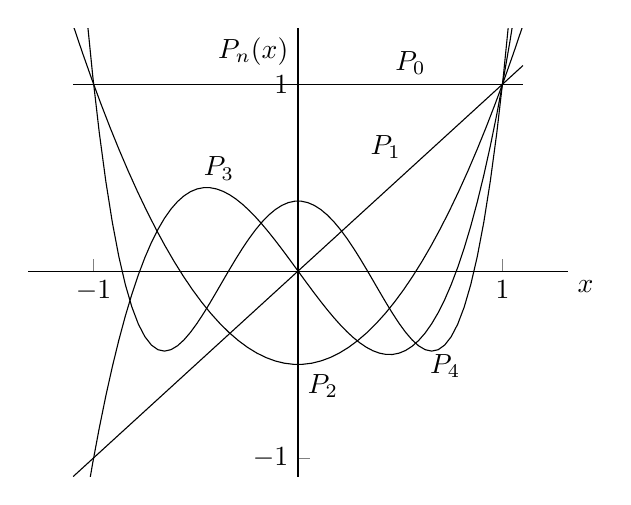
\begin{tikzpicture}
\begin{axis}[axis lines*=middle,ymin=-1.1,ymax=1.3,xlabel={$x$},ylabel={$P_n(x)$},xlabel style={at={(current axis.right of origin)},anchor=north west}, ylabel style={at={(current axis.above origin)},anchor=north east},ylabel style={rotate=-90},ytick={-1,1},yticklabels={$-1$,$1$},xtick={-1,1},xticklabels={$-1$,$1$}]
\pgfmathsetmacro{\lmt}{1.1}
%
\addplot[domain=-\lmt:\lmt]{1}node[pos=0.75,above]{$P_0$};
\addplot[domain=-\lmt:\lmt,samples=50]{1/2*(3*x^2-1)}node[pos=0.5,below right]{$P_2$};
\addplot[domain=-\lmt:\lmt,samples=70]{1/8*(35*x^4-30*x^2+3)}node[pos=0.65,below]{$P_4$};
\addplot[domain=-\lmt:\lmt]{x}node[pos=0.75,above left]{$P_1$};
\addplot[domain=-\lmt:\lmt,samples=70]{1/2*(5*x^3-3*x)}node[pos=0.4,above]{$P_3$};
\end{axis}
\end{tikzpicture}
\caption{لیژانڈر کثیر رکنی۔}
\label{شکل_لیژانڈر_کثیر_رکنی}
\end{figure}

لیژانڈر کثیر رکنی \عددی{P_n(x)} وقفہ \عددی{-1 \le x \le 1} پر آپس میں \اصطلاح{عمودی}\فرہنگ{عمودی}\حاشیہب{orthogonal}\فرہنگ{orthogonal} ہیں۔یہ خصوصیت \اصطلاح{فوریئر لیژانڈر} تسلسل کے لئے ضروری ہے جن پر فوریئر تسلسل کے باب میں غور کیا جائے گا۔
%==============
\ابتدا{مثال}\شناخت{مثال_بیسل_لیژانڈر_عددی_سر}
مساوات \حوالہ{مساوات_بیسل_روایتی_سر_الف} کا دایاں ہاتھ حاصل کریں۔

\انتہا{مثال}
%==========================
